\documentclass[final,hyperref={pdfpagelabels=false},notheorems]{beamer}

\usepackage[orientation=portrait,size=a0,scale=1.3]{beamerposter}

\usetheme{Oxford}

\usepackage[english]{babel}
\usepackage[utf8]{inputenc}
\usepackage{amsmath,amsthm,amssymb,latexsym}
\usepackage{parskip}
\usepackage{graphicx}
\usepackage{amsfonts}
\usepackage{hyperref}
\usepackage[document]{ragged2e}
\usepackage{times}\usefonttheme{professionalfonts}
\usefonttheme[onlymath]{serif}
\usepackage{booktabs}
\usepackage{microtype}
\usepackage{mathtools}
\usepackage{thmtools,thm-restate}
\usepackage{algorithm}
\usepackage[noend]{algpseudocode}
\usepackage[justification=centering,singlelinecheck=false]{caption}
\usepackage{listings}
\usepackage{subcaption}
\usepackage{booktabs}
\usepackage[backend=biber,url=true,doi=true,eprint=false,style=authoryear]{biblatex}

\setlength{\paperwidth}{90cm}
\setlength{\paperheight}{120cm}

\usecaptiontemplate{\small\structure{\insertcaptionname~\insertcaptionnumber: }\insertcaption}

\newcommand{\shrink}{-15pt}

\def\imagetop#1{\vtop{\null\hbox{#1}}}

\addbibresource{references.bib}

\DeclareMathOperator*{\argmin}{arg\,min}
\DeclareMathOperator*{\argmax}{arg\,max}
\DeclareMathOperator*{\Val}{\text{Val}}
\DeclareMathOperator*{\Ch}{\text{Ch}}
\DeclareMathOperator*{\Pa}{\text{Pa}}
\DeclareMathOperator*{\Sc}{\text{Sc}}
\newcommand{\ov}{\overline}
\newcommand{\tsup}{\textsuperscript}

\newtheoremstyle{thesisstyle}
  {5pt}
  {1pt}
  {\itshape}
  {}
  {\bfseries}
  {.}
  {.5em}
  {}

\theoremstyle{thesisstyle}

\newtheorem{definition}{Definition}
\newtheorem{theorem}{Theorem}
\newtheorem{proposition}{Proposition}
\newtheorem{corollary}{Corollary}
\newtheorem{lemma}{Lemma}
\newtheorem{exercise}{Exercise}
\newtheorem{example}{Example}

\newcommand{\set}[1]{\mathbf{#1}}
\newcommand{\pr}{\text{P}}
\newcommand{\eps}{\varepsilon}
\newcommand{\ddspn}[2]{\frac{\partial#1}{\partial#2}}
\newcommand{\iddspn}[2]{\partial#1/\partial#2}
\newcommand{\indep}{\perp}
\renewcommand{\implies}{\Rightarrow}

\newcommand{\bigo}{\mathcal{O}}

\newcommand{\algorithmautorefname}{Algorithm}
\algrenewcommand\algorithmicrequire{\textbf{Input}}
\algrenewcommand\algorithmicensure{\textbf{Output}}

\newcommand{\code}[1]{\lstinline[mathescape=true]{#1}}
\newcommand{\mcode}[1]{\lstinline[mathescape]!#1!}

\newcommand{\pskip}{\vskip 0.5cm}

\title{\huge Mobile Robots Self-Driving Through Image Classification Using Discriminative Learning
of Sum-Product Networks}
\author{\Large Renato Lui Geh (student), Denis Deratani Mauá (advisor)}
\institute{\Large Institute of Mathematics and Statistics, University of São Paulo\\\vspace{4mm}
\texttt{\Large \{renatolg,ddm\}@ime.usp.br}}

\newcommand{\leftfoot}{} % Left footer text
\newcommand{\rightfoot}{} % Right footer text

\makeatletter
\let\@@magyar@captionfix\relax
\makeatother
\begin{document}
\addtobeamertemplate{block end}{}{\vspace*{.05ex}} % White space under blocks
\setbeamertemplate{caption}[numbered]

\begin{frame}[t]

\begin{columns}[t]
  \begin{column}{.015\textwidth}\end{column} % Empty spacer column

%%%%%%%%%%%%%%%%%%%%%%%%%%%%%%%%%%%%%%%%%%
%% Column 1
%%%%%%%%%%%%%%%%%%%%%%%%%%%%%%%%%%%%%%%%%%

  \begin{column}{.5225\textwidth}

    \vspace{\shrink}
    \begin{block}{Motivation and Overview}
      Driving has proven to be a very difficult task for machines to emulate, not only due to the
      inherent complexity of the problem but also because of the need for accurate real-time
      predictions.  Nonetheless, recent advances in computer vision and machine learning have shown
      promising results in the real-world. Mobile robots are low-cost miniature computers with
      limited processing power and memory. The problem of self-driving can be similarly applied to
      the mobile robot domain as a down-scaled version of the same task, with an additional
      hardware constraint. Sum-product networks are probabilistic graphical models capable of
      representing tractable probability distributions containing a great number of variables.
      Exact inference is asymptotically linear to the number of edges in the network's graph, and
      its deep architecture is capable of representing a wide range of distributions. In this work,
      we attempt to model autonomous driving by using sum-product networks on a small mobile robot.
      We model this task as an imitation learning problem through image classification. We present
      accuracy results on an artificial self-driving dataset for different sum-product network
      learning algorithms, providing a comparative study not only for different network
      architectures, but also discriminative and generative models. Finally, we provide a
      real-world mobile robot implementation on a miniature computer.
    \end{block}

    \begin{block}{Sum-Product Networks}
      Sum-product networks are highly expressive deep probabilistic graphical models capable of
      linear time exact inference.
      \begin{definition}[Sum-product network; \cite{gens-domingos}]~\\
        A sum-product network (SPN) is a DAG where each node can be defined recursively as follows.
        \begin{enumerate}
          \item A tractable univariate probability distribution is an SPN\@.
          \item A product of SPNs with disjoint scopes is an SPN\@.
          \item A weighted sum of SPNs with the same scope is an SPN, provided all weights are positive.
          \item Nothing else is an SPN\@.
        \end{enumerate}
      \end{definition}
      Computing the probability of evidence of an SPN given some query variable $X$ and evidence
      $E$ is done by a backward pass through the graph, first computing leaf values and then
      internal nodes until the root is reached. The value of the root $S(X,E)$ is the probability
      $P(X,E)$ as long as all its sum nodes have normalized weights, i.e. they all sum to one.
      \begin{figure}[h]
        \centering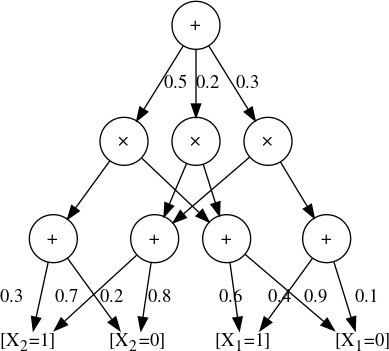
\includegraphics[width=0.5\textwidth]{imgs/sample_spn.png}
        \caption{An SPN with indicator variables as leaves (degenerated univariate distributions).}
      \end{figure}
      This computation is linear in the number of edges, making SPNs an interesting model for
      measuring uncertainty in real-time.
    \end{block}

    \begin{block}{Self-Driving in Mobile Robots}
      Lane tracking is a fundamental aspect of self-driving. The goal of lane tracking in
      self-driving is to correctly identify the road ahead by detecting track marks. Our approach
      to this problem is to make use of imitation learning through image classification, where an
      agent tries to reliably mimick human behavior by classification only. In our case, our
      agent's (i.e. robot's) goal is to remain within the established ``road'' by labelling input
      images as commands for going UP, LEFT or RIGHT. Thus, our objective in this project was to
      build an image classifier capable of accurate predictions in real-time on a miniaturized
      computer.\\~\\

      \begin{figure}
        \begin{subfigure}{0.3\linewidth}
          \centering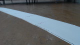
\includegraphics[width=1.0\textwidth]{imgs/sample_left.png}
          \captionsetup{justification=centering}
          \caption*{LEFT}
        \end{subfigure}
        \begin{subfigure}{0.3\linewidth}
          \centering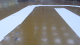
\includegraphics[width=1.0\textwidth]{imgs/sample_up.png}
          \captionsetup{justification=centering}
          \caption*{UP}
        \end{subfigure}
        \begin{subfigure}{0.3\linewidth}
          \centering
\includegraphics[width=1.0\textwidth]{imgs/sample_right.png}
          \captionsetup{justification=centering}
          \caption*{RIGHT}
        \end{subfigure}
        \caption{Dataset samples for lane tracking with their respective labels.}
      \end{figure}
    \end{block}

  \end{column}

%%%%%%%%%%%%%%%%%%%%%%%%%%%%%%%%%%%%%%%%%%
%% Column 2
%%%%%%%%%%%%%%%%%%%%%%%%%%%%%%%%%%%%%%%%%%

  \begin{column}{.02\textwidth}\end{column} % Empty spacer column

  \begin{column}{.5225\textwidth}

    \vspace{\shrink}
    \setbeamertemplate{block begin}[notitle]
    \begin{block}{}
      Our robot consists of two main processing units. The first, nicknamed the Berry, is a
      Raspberry Pi 3 Model B, a Quad Core 1.2GHz Broadcom BCM2837 64bit ARMv7 CPU with 1GB of RAM.
      Coupled with a USB webcam, it is responsible for computing inference and predicting labels.
      The second, named the Brick, is a Lego Mindstorm NXT v2 unit with an Atmel AT91SAM7S256 48MHz
      32bit ARMv4 CPU and 64KB of RAM. It is a dedicated unit for receiving the Berry's commands and
      translating them into motor power.

      \begin{figure}
        \centering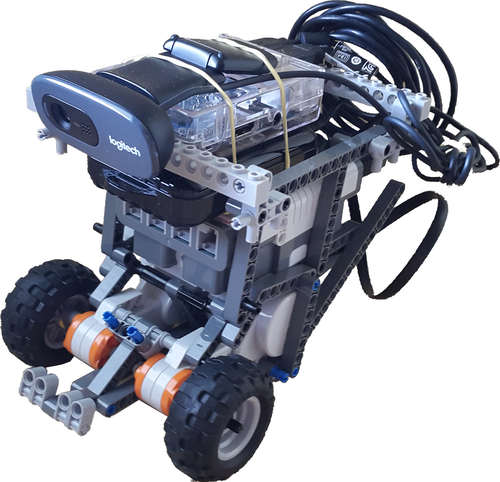
\includegraphics{imgs/robot.png}
        \caption{Fully assembled robot.}
      \end{figure}
    \end{block}
    \setbeamertemplate{block begin}[default]

    \begin{block}{Results}
      The \cite{self-driving} dataset was used for training and testing. It consists of $80\times
      45$ RGB images of road following. We chose to apply some pre-processing to the images, namely
      Otsu's binarization, quantization (i.e. resolution downscaling) and histogram
      equalization.\\~\\
      \begin{figure}
        \begin{subfigure}{0.3\linewidth}
          \centering
\includegraphics[width=\textwidth]{imgs/binary_up.png}
          \captionsetup{justification=centering}
          \caption*{Binarization ($B$)}
        \end{subfigure}
        \begin{subfigure}{0.3\linewidth}
          \centering
\includegraphics[width=\textwidth]{imgs/trans_up.png}
          \captionsetup{justification=centering}
          \caption*{Quantization ($Q_n$)}
        \end{subfigure}
        \begin{subfigure}{0.3\linewidth}
          \centering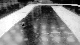
\includegraphics[width=\textwidth]{imgs/eq_up.png}
          \captionsetup{justification=centering}
          \caption*{Equalization ($E$)}
        \end{subfigure}
        \caption{Image transformations done before training and inference.}
      \end{figure}
      We trained the SPNs with two structure learning algorithms: \cite{gens-domingos}
      (\textbf{GD}), \cite{clustering} (\textbf{DV}); and performed generative (\textbf{g}) and
      discriminative (\textbf{d}) gradient descent weight learning on both architectures. We
      additionally generated the structures with no weight learning (\textbf{s}) as a form of
      control.\\~\\
      \begin{table}[h]
        \centering
        \begin{tabular}{l|c|c|c|c|c|c}
          \hline
          \multicolumn{1}{c}{\bfseries (\%, secs)} & \multicolumn{1}{c}{\bfseries DV+g} &
          \multicolumn{1}{c}{\bfseries DV+d} & \multicolumn{1}{c}{\bfseries DV+s} &
          \multicolumn{1}{c}{\bfseries GD+g} & \multicolumn{1}{c}{\bfseries GD+d} &
          \multicolumn{1}{c}{\bfseries GD+s}\\
          \hline
          $B$         & (78.8, 0.23) & (78.8, 0.25) & (78.8, 0.25) & (82.8, 0.38) & (83.8, 0.37) & (85.0, 0.31)\\
          $Q_2$       & (78.6, 0.22) & (78.0, 0.24) & (78.0, 0.23) & (78.6, 0.28) & (80.4, 0.34) & (79.4, 0.16)\\
          $Q_2+E$     & (76.6, 0.22) & (76.6, 0.23) & (76.8, 0.23) & (79.6, 0.38) & (82.8, 0.30) & (81.8, 0.27)\\
          $Q_4$       & (78.2, 0.22) & (78.4, 0.22) & (78.2, 0.23) & (76.0, 0.16) & (78.2, 0.17) & (76.4, 0.13)\\
          $Q_4+E$     & (76.6, 0.23) & (76.6, 0.27) & (76.8, 0.29) & (76.0, 0.13) & (74.6, 0.14) & (80.6, 0.13)\\
          $Q_6$       & (77.4, 0.23) & (78.4, 0.24) & (78.4, 0.23) & (75.2, 0.04) & (74.4, 0.05) & (72.0, 0.01)\\
          $Q_6+E$     & (76.0, 0.22) & (76.4, 0.24) & (76.4, 0.28) & (73.0, 0.03) & (75.0, 0.04) & (73.6, 0.02)\\
          $\emptyset$ & (78.0, 0.22) & (78.4, 0.26) & (78.4, 0.23) & (62.4, 0.02) & (62.4, 0.01) & (62.4, 0.01)\\
          $E$         & (76.4, 0.23) & (76.4, 0.23) & (76.4, 0.22) & (60.4, 0.01) & (60.0, 0.01) & (61.2, 0.02)\\
        \end{tabular}
        \caption{Accuracy values in percentage and inference time in seconds for each possible model
        permutation.\label{tab:accuracy}}
      \end{table}
      Table \ref{tab:accuracy} shows results for each model and the pre-process filter applied
      beforehand. In this table we only show even quantizations.\\~\\

      We also applied the model to a real-world application: \url{https://youtu.be/}
    \end{block}

    \begin{block}{Conclusions}
      Sum-product networks were able to somewhat accurately predict the labels. Because of fast
      inference, prediction error was smoothed out, as the model was capable of correcting itself
      every hundred milliseconds. Network complexity also played a huge factor in prediction, as a
      deeper, more complex model achieved better theoretical accuracy, but took longer to predict.
      This tradeoff can become troublesome, as a self-driving vehicle must be able to predict and
      correct itself at least as fast as a human. Overall, the model was able to navigate the track
      reasonably well for a primitive form of control.
    \end{block}

    \begin{block}{References}
      \linespread{0.928}\selectfont
      %\footnotesize{\bibliographystyle{unsrt}
      %\bibliography{references}}
      \printbibliography[heading=none]
    \end{block}

  \end{column}

  \begin{column}{.015\textwidth}\end{column} % Empty spacer column

\end{columns} % End of all the columns in the poster

\end{frame} % End of the enclosing frame

\end{document}
